\documentclass[a4paper,10pt]{article}
 
\usepackage[T1]{fontenc}
\usepackage[utf8]{inputenc}
\usepackage{graphicx}
\usepackage{xcolor, colortbl}
\usepackage{caption}
\usepackage{hyperref}
\usepackage{listings}
\usepackage{wrapfig} 
\usepackage{tabu} % For coloring single row of table

\renewcommand\familydefault{\sfdefault} 
\usepackage{tgheros}
\usepackage[defaultmono]{droidmono}

\usepackage{amsmath,amssymb,amsthm,textcomp}
\usepackage{enumerate}
\usepackage{multicol}
\usepackage{tikz}

\usepackage{geometry}
\usepackage{trace}
\usepackage{tcolorbox}
\usepackage{tabularx}
\usepackage{accsupp}% http://ctan.org/pkg/accsupp


\tcbuselibrary{listings,skins} % For lstlisting

\geometry{total={210mm,297mm},
left=25mm,right=25mm,%
bindingoffset=0mm, top=20mm,bottom=20mm}


% For coloring single row in table
\def\zapcolorreset{\let\reset@color\relax\ignorespaces}
\def\colorrows#1{\noalign{\aftergroup\zapcolorreset#1}\ignorespaces}

%\linespread{1.3}

\newcommand{\linia}{\rule{\linewidth}{0.5pt}}
\newcommand{\ano}{\text{1}}

% custom theorems if needed
\newtheoremstyle{mytheor}
    {1ex}{1ex}{\normalfont}{0pt}{\scshape}{.}{1ex}
    {{\thmname{#1 }}{\thmnumber{#2}}{\thmnote{ (#3)}}}

\theoremstyle{mytheor}
\newtheorem{defi}{Definition}

% my own titles
\makeatletter
\renewcommand{\maketitle}{
\begin{center}
\vspace{2ex}
{\huge \textsc{\@title}}
\vspace{1ex}
\\
ECN 104  - Digital Logic Design \\
Department of Electronics and Communication Engineering \\
Indian Institute of Technology, Roorkee
\linia\\
\@author \hfill \@date
\vspace{4ex}
\end{center}
}
\makeatother
%%%

% custom footers and headers
\usepackage{fancyhdr}
\pagestyle{fancy}
\lhead{}
\chead{}
\rhead{}
\lfoot{Assignment \ano - Introduction to Verilog}
\cfoot{}
\rfoot{Page \thepage}
\renewcommand{\headrulewidth}{0pt}
\renewcommand{\footrulewidth}{0pt}
%

\definecolor{vgreen}{RGB}{104,180,104}
\definecolor{vblue}{RGB}{49,49,255}
\definecolor{vorange}{RGB}{255,143,102}

\makeatletter
\newcommand*\@lbracket{[}
\newcommand*\@rbracket{]}
\newcommand*\@colon{:}
\newcommand*\colorIndex{%
    \edef\@temp{\the\lst@token}%
    \ifx\@temp\@lbracket \color{black}%
    \else\ifx\@temp\@rbracket \color{black}%
    \else\ifx\@temp\@colon \color{black}%
    \else \color{vorange}%
    \fi\fi\fi
}
\makeatother

\definecolor{codebg}{RGB}{250,250,240} 
\definecolor{greatblue}{RGB}{91,155,215} 

% Set up caption and labels for lstlistings
\DeclareCaptionFont{white}{\color{white}}
\DeclareCaptionFormat{listing}{\colorbox{greatblue}{\parbox{\textwidth}{\hspace{1cm}#1#2#3}}}
\captionsetup[lstlisting]{format=listing,labelfont=white,textfont=white}

\renewcommand{\thelstnumber}{% Line number printing mechanism
  \protect\BeginAccSupp{ActualText={}}\arabic{lstnumber}\protect\EndAccSupp{}%
}

\def\backtick{\char18} 
\lstdefinestyle{verilog-style}
{
    %columns=fullflexible, 
    language=Verilog,
    basicstyle=\small\ttfamily,
    keywordstyle=\color{vblue},
    identifierstyle=\color{black},
    commentstyle=\color{vgreen},
    numbers=left, 
    numberstyle=\color{gray},  
    numbersep=10pt,
    moredelim=*[s][\colorIndex]{[}{]},
    literate=*{:}{:}1, 
    backgroundcolor=\color{codebg},
    framexrightmargin=0.09cm, 
    framexleftmargin=-0.09cm,
    frame=trbl,
    upquote=true, 
    framerule=0pt,
    keepspaces=true
}

\newcommand{
  \insertverilog}[3]{
  \lstinputlisting[label=#2, caption=#3, style={verilog-style}]{#1}
}


%%%----------%%%----------%%%----------%%%----------%%%
% Command for creating a resource box
\newcommand{\resourcebox}[2]{
  \fbox{%
    \parbox{0.5\textwidth}{%
      \text{#1}
    }%
  } 
}


%%%----------%%%----------%%%----------%%%----------%%%

\makeatletter
\def\lst@outputspace{{\ifx\lst@bkgcolor\empty\color{white}\else\lst@bkgcolor\fi\lst@visiblespace}}
\makeatother


%%%----------%%%----------%%%----------%%%----------%%%
\begin{document}

\title{Assignment \ano \\ Introduction to Verilog}

\maketitle

\section*{Hardware Description Languages}
Hardware description language (HDL) is a convienient, device and technology independent way of representing digital logic. HDLs are helpful describing, simulating and verifying digital circuits.

\subsection*{Why not use C/C++, Java...?} 
C/C++, Java are programming languages which are very good at what they were designed for, that is programming. However describing digital circuits in programming language is difficult and often confusing, which led to development of HDLs.

\subsection*{Which HDL to use?}
Today many Hardware description languages are available, each of them are different from each other in terms of functionality, semantic and grammar. In this course however we will be using Verilog  2001.

\section*{Using Verilog 2001}
As a begininer we are going to describe and simulate simple combinational circuit with Verilog.

\section*{Design Flow}  

\begin{figure}[!t] \centering 
  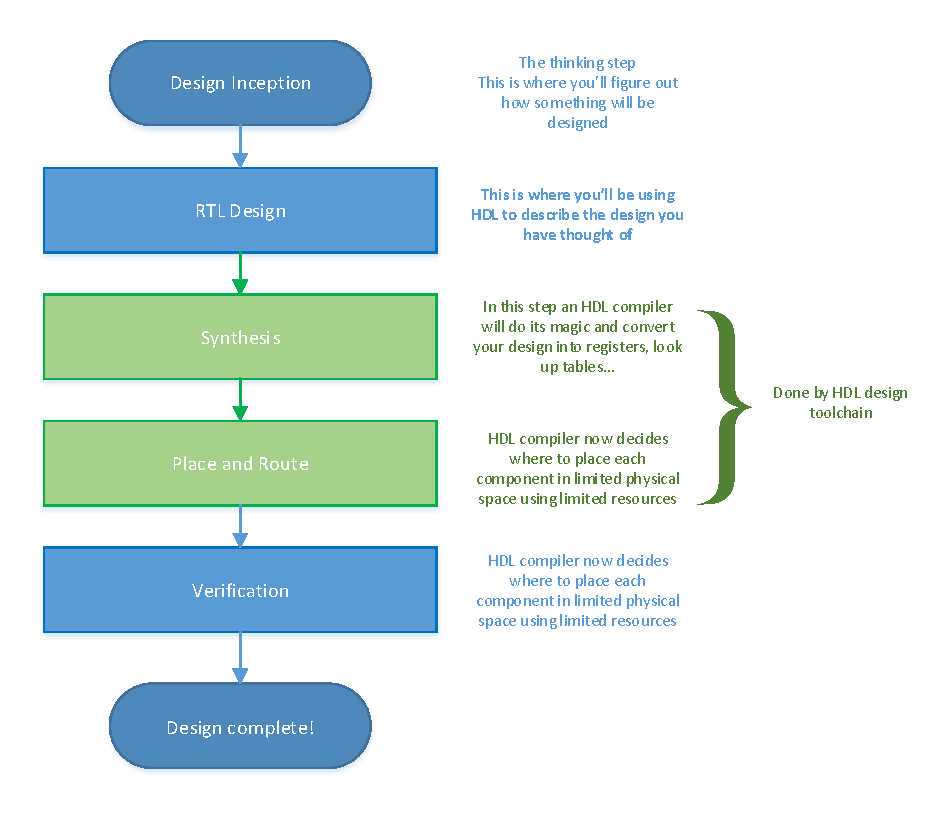
\includegraphics[width=\linewidth]{./resources/hdl_design_flow.pdf}
  \caption{Example binary search tree constructed using names from Table \ref{Table:ndn_name_table} with insertion order and output port information.}
  \label{Fig:bst_sample_names}
\end{figure} 

\section*{Verilog Syntax}
\subsection*{Modules}
Module is the basic building block in Verilog, modules helps in organizing and structuring designs in logical and human readable form. Module can be considered as analogus to functions in programming languages.

\insertverilog{./verilog_files/module.v}{sample-module}{\text{Sample module indicating its structure}}

An example of AND gate would be
\insertverilog{./verilog_files/andGate.v}{sample-module}{\text{Illustrative AND gate module}}

\subsection*{Instantiating modules}
The process of creating objects of modules is called instatiation in Verilog. Modules are a
  
\insertverilog{./verilog_files/AndGate3.v}{sample-module}{\text{Illustrative AND gate module}} 
\subsection*{Comments}
Comments in verilog are of two kinds:
\subsubsection*{Single Line Comment}
Two forward slashes represents begining of a single line comment in verilog, any charater after the two forward slashes will be ignored by verilog compiler until the end of line.
\insertverilog{./verilog_files/singleLineComment.v}{single-line-comment}{\text{Single line comment}} 

\subsubsection*{Block Comment}
Block comments in verilog are used to comment more than one line, the start with `/*' and ends with `*/'. Anything between these two character sequence is ignored by the compiler.
\insertverilog{./verilog_files/blockComment.v}{block-comment}{\text{Block
    comment}}

\subsection*{Numerical Literals}
\subsubsection*{Sized Numbers}
To represent digital circuits accurately Verilog allows defining
numbers of fixed size. These numbers have following format:
\begin{center}
  <size>'<character for base><number>
\end{center}

For example:
\insertverilog{./verilog_files/sizedNumbers.v}{sized-numbers}{\text{Example of sized numbers}}
 
\subsubsection*{Unisized Numbers}
Verilog also includes support for unsized numbers. These numbers are
assumed to be of a particular size depending upon the
compiler/machine.

\subsection*{Constants}
Global constants can be decalered in Verilog. When Verilog code is processed all these constants will be replaced by their respective values. NOTE: Verilog constants always starts with backtick ` ${}^{\backprime}$ '. 
\insertverilog{./verilog_files/constants.v}{constants}{\text{Declaration and use of constants}}

\subsection*{Wires}

\begin{figure}[!h] \centering  
  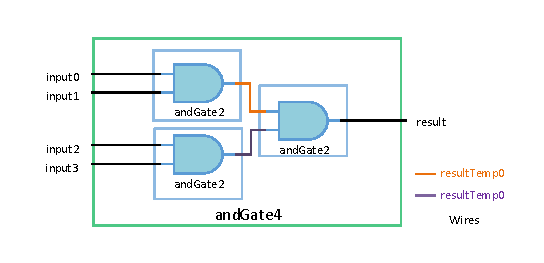
\includegraphics[width=\linewidth]{./resources/andGate4_representation.pdf}
  \caption{Gate level representation of code in Listing \ref{andGate4-wire}.} 
  \label{Fig:andGate4-representation}
\end{figure}

Wires are something very important in verilog, use of wires in Verilog is for what wires are used in real life ... to connect two things electrically! Wires will be used extensively in future assignments to connect two modules, registers and even wires together. This concept is explained using Listing \ref{constants} where wires are used to connect output of two 2-input AND gates to inputs of single 2-input AND gates. Gate level diagram of which is shown in Fig. \ref{Fig:andGate4-representation}.

\insertverilog{./verilog_files/andGate4.v}{andGate4-wire}{\text{Use of wires to connect output of one module to input of another}}

\subsubsection*{Vectors}
Verilog support declaration of wire to represent group of wires (or registers which will be explained later). Vectors are declared by specifying their type, range and then their name:
\begin{center}
  <type> <range> <name>;
\end{center}

Example declaration of 6 bit wide vector of type wire:
\begin{center}
  {\color{blue} wire} [{\color{orange}5}:{\color{orange}0}] new\_wire; {\color{vgreen}// Both the range specifier digits are inclusive}
\end{center}

Here new\_wire[{\color{orange}5}] is MSB while new\_wire[{\color{orange}0}] is LSB.
\subsection*{Operators}
Verilog supports wide range of operators to represent mathematical operations, these are high level representation of what would be converted to gate level implementation later by the HDL compiler.

\begin{table}[h]
  \begin{center}
    \label{Table:operators-table}
    \caption{List of common operators used in Verilog}
    \renewcommand{\arraystretch}{1.1}
    \begin{tabularx}{.8\textwidth}{|X|X|X|} 
      \hline
      \rowcolor{greatblue}
      \color{white}  Operator & \color{white}Description & \color{white}Functional Group \\
      %  \colorrows{\color{black}} 
      \hline
      \text{[]} & bit select or part select &  \\
      
      \hline
      \text{()} & parenthesis &  \\
      
      \hline
      \text{!} & negation &  logical\\
      \text{\textasciitilde} & negation &  bit\-wise\\
      \text{\&} & reduction AND & reduction \\
      \text{\textbar} & reduction OR & reduction \\
      \text{\textasciitilde\&} & reduction NAND & reduction \\
      \text{\textasciitilde\textbar} & reduction NOR & reduction \\
      $^\wedge$ & reduction XOR & reduction \\
      \textasciitilde$^\wedge$ or $^\wedge$\textasciitilde & reduction XNOR & reduction \\
      \hline
      $+$ & Unary Plus (plus sign) & airthmetic \\
      $-$ & Unary minus (minus sign) & \\
      \hline
      $*$ & multiply & airthmetic \\
      $/$ & divide &  \\
      \% & modulus &  \\
      \hline
      $+$ & Binary Plus & airthmetic \\
      $-$ & Binary minus &  \\
      \hline
      $<<$ & shift left & shift \\
      $>>$ & shift right &  \\
      \hline
      $>$ & greater than & relational \\
      $>=$  & greater than or equal to & \\
      $<$ & less than  & \\
      $<=$ & less than or equal to & \\
      \hline  
      $==$ & case equality & equality \\
      $!=$  & case inequality & \\
      \hline
      \text{\&} & bitwise AND & bitwise \\
      \text{\textbar} & bitwise OR & \\
      \text{\textasciitilde} & bitwise XOR & \\
      \hline
    \end{tabularx}
  \end{center}
\end{table}

\subsubsection*{Airthmetic Operators}
Veriog allows use of various airthmetic operators to perform
calculations on vectors (wires \& reg). Following example shows its
usage:
\insertverilog{./verilog_files/airthmeticOperators.v}{airthmetic-operators}{\text{Functioning of airthmetic operator}}

\subsubsection*{Reduction Operators}
Reduction operators in Verilog reduces a multibit number into a single
bit by repeatedly performing a specified operation. Following example 
explains its usage: 
\insertverilog{./verilog_files/reductionOperators.v}{reduction-operators}{\text{Functioning of reduction operator}}
 
\subsubsection*{Relational Operators}
Relational operators in verilog are used to compare two values, usage
of all four type of relational operators supported by Verilog are
given in Listing \ref{relational-operators}.
\insertverilog{./verilog_files/relationalOperators.v}{relational-operators}{\text{Functioning of relational operator}}
  
\subsubsection*{Logical Operators}
Logical operators are used in conjuction with relational and equality
to perform multiple comparisions within a single expression.
Example usage of logical operators are provided in listing  \ref{logical-operators}.
\insertverilog{./verilog_files/logicalOperators.v}{logical-operators}{\text{Functioning of logical operator}}

\subsubsection*{Bitwise and Shift Operators}
Verilog Bitwise and Shift operators works in the same way as they work
in Java, except that in Verilog only left shift ($<<$) and right shift
($>>$) are supported.

\section*{Problems}
\subsection*{Problem 1:}
Design a 16 input AND gate using Verilog reduction operator where input to the module will be a vector of length 16 and will have a single output.
Use the code in Listing \ref{question1}. 
\insertverilog{./verilog_files/question1.v}{question1}{\text{Question 1}}

\subsection*{Problem 2:}
Design a 4 input AND gate using Verilog reduction operator where input to the module will be a vector of length 4 and will have a single output.
\subsection*{Problem 3:}
Design a 4 input AND gate using Verilog reduction operator where input to the module will be a vector of length 4 and will have a single output.
\subsection*{Problem 4:}
Design a 4 input AND gate using Verilog reduction operator where input to the module will be a vector of length 4 and will have a single output.
\subsection*{Problem 5:}
Make a module for 2 input NAND gate. Now, make a 2 input And gate by connecting both the input of NAND gate to another NAND gate.


\section*{References}
\begin{itemize}
  \item \url{http://cva.stanford.edu/people/davidbbs/classes/ee108a/winter0607\%20labs/ee108a\_nham\_intro\_to\_verilog.pdf}
  \item Verilog HDL \- Samir Palnitkar
  \item \url{https://www.utdallas.edu/\~akshay.sridharan/index\_files/Page5212.html}
\end{itemize}


\end{document}
